%\documentclass[12pt]{article}

\newcommand{\he}{\hat{\mathbf{e}}}

\questionheader{ex:s1.8}

%%%%%%%%%%%%%%%%%%
\subsection*{\Conceptual}
%%%%%%%%%%%%%%%%%%

%%%%%%%%%%%%%%%%%%%%%%%%%%%
\begin{question}
Consider the points
\begin{align*}
(x_1,y_1) &= (3,0) &
(x_2,y_2) &= (1,1)  &
(x_3,y_3) &= (0,1) \\
(x_4,y_4) &= (-1,1) &
(x_5,y_5) &= (-2,0)
\end{align*}
For each $1\le i\le 5$, 
\begin{itemize}
\item
sketch, in the $xy$-plane, the point $(x_i,y_i)$ and
\item
find the polar coordinates $r_i$ and $\theta_i$,
with $0\le\theta_i<2\pi$, for the point $(x_i,y_i)$.
\end{itemize}
\end{question}

%\begin{hint} 
%\end{hint}

\begin{answer} 
The left hand sketch below contains the points, $(x_1,y_1)$, $(x_3,y_3)$,
$(x_5,y_5)$, that are on the axes. The right hand sketch below contains the
points, $(x_2,y_2)$, $(x_4,y_4)$, that are not on the axes.
\begin{center}
  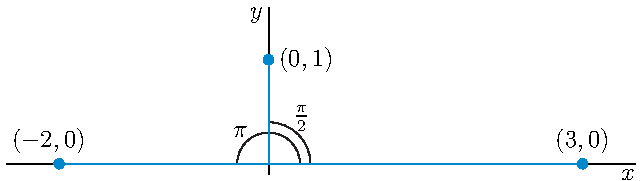
\includegraphics[scale=0.95]{polar3A.pdf}\quad
  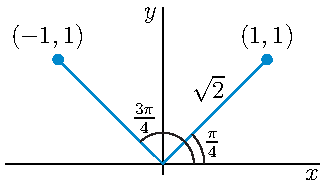
\includegraphics[scale=0.95]{polar2A.pdf}
\end{center}
    $r_1 = 3$,        $\theta_1=0$\qquad 
    $r_2 = \sqrt{2}$, $\theta_2=\frac{\pi}{4}$\qquad 
    $r_3 = 1$,        $\theta_3=\frac{\pi}{2}$\qquad 
    $r_4 = \sqrt{2}$, $\theta_4=\frac{3\pi}{4}$\\
    $r_5 = 2$,        $\theta_5=\pi$
\end{answer}


\begin{solution}
The left hand sketch below contains the points, $(x_1,y_1)$, $(x_3,y_3)$,
$(x_5,y_5)$, that are on the axes. The right hand sketch below contains the
points, $(x_2,y_2)$, $(x_4,y_4)$, that are not on the axes.
\begin{center}
  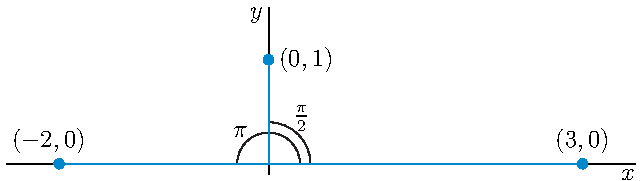
\includegraphics[scale=0.95]{polar3A.pdf}\quad
  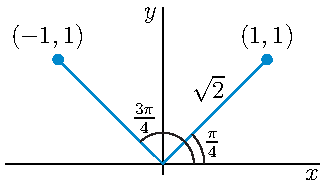
\includegraphics[scale=0.95]{polar2A.pdf}
\end{center}
Recall that the polar coordinates $r$, $\theta$
are related to the cartesian coordinates $x$, $y$, by $x=r\cos\theta$,
$y=r\sin\theta$. So $r=\sqrt{x^2+y^2}$ and $\tan\theta=\frac{y}{x}$
(assuming that $x\ne 0$) and
\begin{alignat*}{5}
(x_1,y_1) &= (3,0) &&\implies &r_1=3,\ \tan\theta_1=0
                   &&\implies \theta_1&=0 
                   \text{ as $(x_1,y_1)$ is on the positive $x$-axis} \\
(x_2,y_2) &= (1,1) &&\implies &r_2=\sqrt{2},\ \tan\theta_2=1
                   &&\implies \theta_2&=\frac{\pi}{4} 
                   \text{ as $(x_2,y_2)$ is in the first octant} \\
(x_3,y_3) &= (0,1) &&\implies &r_3=1,\ \cos\theta_3=0
                   &&\implies \theta_3&=\frac{\pi}{2} 
                   \text{ as $(x_3,y_3)$ is on the positive $y$-axis} \\
(x_4,y_4) &= (-1,1) &&\implies &r_4=\sqrt{2},\ \tan\theta_4=-1
                   &&\implies \theta_4&=\frac{3\pi}{4} 
                   \text{ as $(x_4,y_4)$ is in the third octant} \\
(x_5,y_5) &= (-2,0) &&\implies &r_5=2,\ \tan\theta_5=0
                   &&\implies \theta_5&=\pi 
                   \text{ as $(x_5,y_5)$ is on the negative $x$-axis} 
\end{alignat*}
\end{solution}


%%%%%%%%%%%%%%%%%%%%%%%%%%%
\begin{question}
\begin{enumerate}[(a)]
\item
Find \emph{all} pairs $(r,\theta)$ such that
\begin{equation*}
(-2,0) = \big(r\cos\theta\,,\,r\sin\theta\big)
\end{equation*}
\item
Find \emph{all} pairs $(r,\theta)$ such that
\begin{equation*}
(1,1) = \big(r\cos\theta\,,\,r\sin\theta\big)
\end{equation*}
\item
Find \emph{all} pairs $(r,\theta)$ such that
\begin{equation*}
(-1,-1) = \big(r\cos\theta\,,\,r\sin\theta\big)
\end{equation*}
\end{enumerate}
\end{question}

\begin{hint} 
$r$ is allowed to be negative.
\end{hint}

\begin{answer} 
(a) $\big(r=2\,,\,\theta= n\pi,\ n\text{ odd integer }\big)$ or 
    $\big(r=-2\,,\,\theta= n\pi,\ n\text{ even integer }\big)$ 

(b) $\big(r=\sqrt{2}\,,\,\theta= \nicefrac{\pi}{4} + 2n\pi\big)$ or 
    $\big(r=-\sqrt{2}\,,\,\theta= \nicefrac{5\pi}{4} + 2n\pi\big)$,
    with $n$ integer. 

(c) $\big(r=\sqrt{2}\,,\,\theta= \nicefrac{5\pi}{4} + 2n\pi\big)$ or 
    $\big(r=-\sqrt{2}\,,\,\theta= \nicefrac{\pi}{4} + 2n\pi\big)$,
    with $n$ integer. 
\end{answer}


\begin{solution}
Note that the distance from the point $\big(r\cos\theta\,,\,r\sin\theta\big)$
to the origin is
\begin{equation*}
\sqrt{r^2\cos^2\theta + r^2\sin^2\theta}
=\sqrt{r^2}
=|r|
\end{equation*}
Thus $r$ can be either the distance to the origin or minus the distance to the
origin.

(a) 
The distance from $(-2,0)$ to the origin is $2$. So either $r=2$ or $r=-2$.
\begin{itemize}
\item If $r=2$, then $\theta$ must obey 
\begin{align*}
(-2,0) = \big(2\cos\theta\,,\,2\sin\theta\big)
&\iff \sin\theta=0,\ \cos\theta=-1 \\
&\iff \theta= n\pi,\ n\text{ integer },\ \cos\theta=-1 \\
&\iff \theta= n\pi,\ n\text{ odd integer }
\end{align*}
\item If $r=-2$, then $\theta$ must obey 
\begin{align*}
(-2,0) = \big(-2\cos\theta\,,\,-2\sin\theta\big)
&\iff \sin\theta=0,\ \cos\theta=1 \\
&\iff \theta= n\pi,\ n\text{ integer },\ \cos\theta=1 \\
&\iff \theta= n\pi,\ n\text{ even integer }
\end{align*}
\end{itemize}
In the figure on the left below, the blue half-line is the set of all points 
with polar coordinates $\theta=\pi$, $r>0$ and the pink half-line is the set 
of all points  with polar coordinates $\theta=\pi$, $r<0$. 
In the figure on the right below, the blue half-line is the set of all points 
with polar coordinates $\theta=0$, $r>0$ and the pink half-line is the set 
of all points  with polar coordinates $\theta=0$, $r<0$. 
\begin{center}
  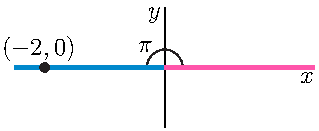
\includegraphics{polar6B.pdf}\qquad
  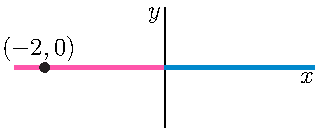
\includegraphics{polar6A.pdf}
\end{center}


(b)
The distance from $(1,1)$ to the origin is $\sqrt{2}$. 
So either $r=\sqrt{2}$ or $r=-\sqrt{2}$.
\begin{itemize}
\item If $r=\sqrt{2}$, then $\theta$ must obey 
\begin{align*}
(1,1) = \big(\sqrt{2}\,\cos\theta\,,\,\sqrt{2}\,\sin\theta\big)
&\iff \sin\theta=\cos\theta=\nicefrac{1}{\sqrt{2}} \\
&\iff \theta= \nicefrac{\pi}{4} + 2n\pi,\ n\text{ integer }
\end{align*}
\item If $r=-\sqrt{2}$, then $\theta$ must obey 
\begin{align*}
(1,1) = \big(-\sqrt{2}\,\cos\theta\,,\,-\sqrt{2}\,\sin\theta\big)
&\iff \sin\theta=\cos\theta=-\nicefrac{1}{\sqrt{2}} \\
&\iff \theta= \nicefrac{5\pi}{4} + 2n\pi,\ n\text{ integer }
\end{align*}
\end{itemize}
In the figure on the left below, the blue half-line is the set of all points 
with polar coordinates $\theta=\frac{\pi}{4}$, $r>0$ and the pink half-line 
is the set of all points  with polar coordinates $\theta=\frac{\pi}{4}$, $r<0$. 
In the figure on the right below, the blue half-line is the set of all points 
with polar coordinates $\theta=\frac{5\pi}{4}$, $r>0$ and the pink 
half-line is the set of all points  with polar coordinates 
$\theta=\frac{5\pi}{4}$, $r<0$. 
\begin{center}
  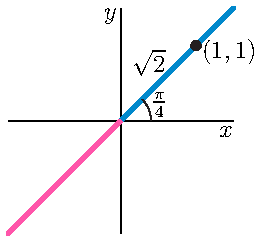
\includegraphics{polar4A.pdf}\qquad
  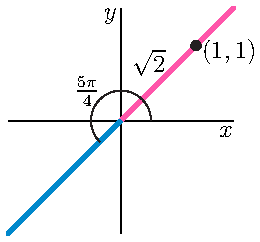
\includegraphics{polar4B.pdf}
\end{center}

(c)
The distance from $(-1,-1)$ to the origin is $\sqrt{2}$. 
So either $r=\sqrt{2}$ or $r=-\sqrt{2}$.
\begin{itemize}
\item If $r=\sqrt{2}$, then $\theta$ must obey 
\begin{align*}
(-1,-1) = \big(\sqrt{2}\,\cos\theta\,,\,\sqrt{2}\,\sin\theta\big)
&\iff \sin\theta=\cos\theta=-\nicefrac{1}{\sqrt{2}} \\
&\iff \theta= \nicefrac{5\pi}{4} + 2n\pi,\ n\text{ integer }
\end{align*}
\item If $r=-\sqrt{2}$, then $\theta$ must obey 
\begin{align*}
(-1,-1) = \big(-\sqrt{2}\,\cos\theta\,,\,-\sqrt{2}\,\sin\theta\big)
&\iff \sin\theta=\cos\theta=\nicefrac{1}{\sqrt{2}} \\
&\iff \theta= \nicefrac{\pi}{4} + 2n\pi,\ n\text{ integer }
\end{align*}
\end{itemize}
In the figure on the left below, the blue half-line is the set of all points 
with polar coordinates $\theta=\frac{5\pi}{4}$, $r>0$ and the pink half-line 
is the set of all points  with polar coordinates 
$\theta=\frac{5\pi}{4}$, $r<0$. 
In the figure on the right below, the blue half-line is the set of all points 
with polar coordinates $\theta=\frac{\pi}{4}$, $r>0$ and the pink 
half-line is the set of all points  with polar coordinates 
$\theta=\frac{\pi}{4}$, $r<0$. 
\begin{center}
  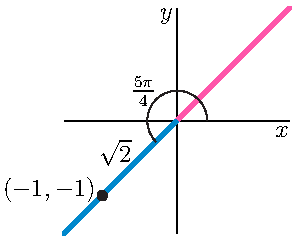
\includegraphics{polar5A.pdf}\qquad
  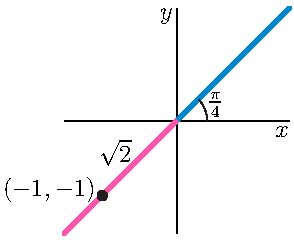
\includegraphics{polar5B.pdf}
\end{center}

\end{solution}



%%%%%%%%%%%%%%%%%%%%%%%%%%%
\begin{question}\label{prb polar vectors}
Consider the points
\begin{align*}
(x_1,y_1) &= (3,0) &
(x_2,y_2) &= (1,1)  &
(x_3,y_3) &= (0,1) \\
(x_4,y_4) &= (-1,1) &
(x_5,y_5) &= (-2,0)
\end{align*}
Also define, for each angle $\theta$, the vectors
\begin{align*}
\he_r(\theta)=\cos\theta\ \hi + \sin\theta\ \hj\qquad
\he_\theta(\theta) = -\sin\theta\ \hi + \cos\theta\ \hj
\end{align*}
\begin{enumerate}[(a)]
\item
Determine, for each angle $\theta$, the lengths of the vectors
$\he_r(\theta)$ and $\he_\theta(\theta)$ and the angle between 
the vectors $\he_r(\theta)$ and $\he_\theta(\theta)$. Compute
$\he_r(\theta)\times\he_\theta(\theta)$ (viewing $\he_r(\theta)$ and $\he_\theta(\theta)$ as vectors in three dimensions with zero $\hk$ 
components).
\item
For each $1\le i\le 5$, sketch, in the $xy$-plane, the point $(x_i,y_i)$
and the vectors $\he_r(\theta_i)$ and $\he_\theta(\theta_i)$. In your
sketch of the vectors, place the tails of the vectors 
$\he_r(\theta_i)$ and $\he_\theta(\theta_i)$ at $(x_i,y_i)$.
\end{enumerate}
\end{question}

\begin{hint} 
Compute, for each angle $\theta$, the dot product $\he_r(\theta)\cdot\he_\theta(\theta)$.
\end{hint}

\begin{answer} 
(a) Both $\he_r(\theta)$ and $\he_\theta(\theta)$ have length 1.
The angle between them is $\frac{\pi}{2}$. The cross product is
$\he_r(\theta) \times \he_\theta(\theta)=\hk$.

(b)
Here is a sketch of $(x_i,y_i)$, $\he_r(\theta_i)$,
$\he_\theta(\theta_i)$ for $i =1,3,5$ (the points on the axes)
\begin{center}
  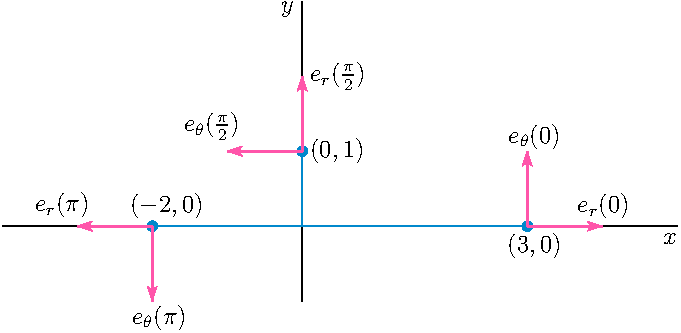
\includegraphics{polar3.pdf}
\end{center}
and here is a sketch (to a different scale) of $(x_i,y_i)$, $\he_r(\theta_i)$,
$\he_\theta(\theta_i)$ for $i =2,4$ (the points off the axes).
\begin{center}       
  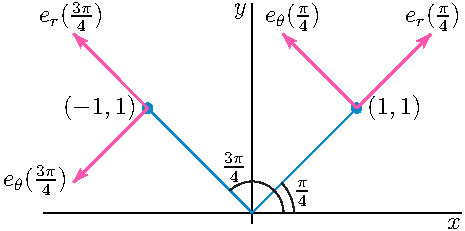
\includegraphics{polar2.pdf}
\end{center}
\end{answer}


\begin{solution} 
(a) The lengths are
\begin{align*}
|\he_r(\theta)| &= \sqrt{\cos^2\theta+\sin^2\theta} = 1 \\
|\he_\theta(\theta)| &= \sqrt{(-\sin\theta)^2+\cos^2\theta} = 1 
\end{align*}
As 
\begin{equation*}
\he_r(\theta) \cdot \he_\theta(\theta) = (\cos\theta)(-\sin\theta)
                                        +(\sin\theta)(\cos\theta)=0
\end{equation*}
the two vectors are perpendicular and the angle between them is 
$\frac{\pi}{2}$. The cross product is
\begin{align*}
\he_r(\theta) \times \he_\theta(\theta)
&=\det\left[\begin{matrix}
                  \hi  &  \hj        & \hk \\
           \cos\theta  & \sin\theta  &  0  \\
          -\sin\theta  & \cos\theta  &  0
            \end{matrix}\right] =\hk
\end{align*}

(b) Note that for $\theta$ determined by $x=r\cos\theta$, $y=r\sin\theta$,
\begin{itemize}\itemsep1pt \parskip0pt \parsep0pt %\itemindent-15pt
\item
the vector $\he_r(\theta)$ is a unit vector in the same direction as the
vector from $(0,0)$ to $(x,y)$ and 
\item
the vector $\he_\theta(\theta)$ is a unit vector that is perpendicular 
to $\he_r(\theta)$. 
\item
The $y$-component of $\he_\theta(\theta)$ has the same sign 
as the $x$-component of $\he_r(\theta)$.
The $x$-component of $\he_\theta(\theta)$ has opposite sign to that of the $y$-component  of $\he_r(\theta)$. 
\end{itemize}
Here is a sketch of $(x_i,y_i)$, $\he_r(\theta_i)$,
$\he_\theta(\theta_i)$ for $i =1,3,5$ (the points on the axes)
\begin{center}
  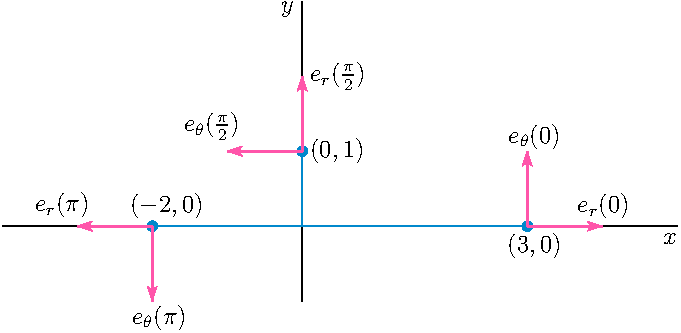
\includegraphics{polar3.pdf}
\end{center}
and here is a sketch (to a different scale) of $(x_i,y_i)$, $\he_r(\theta_i)$,
$\he_\theta(\theta_i)$ for $i =2,4$ (the points off the axes).
\begin{center}       
  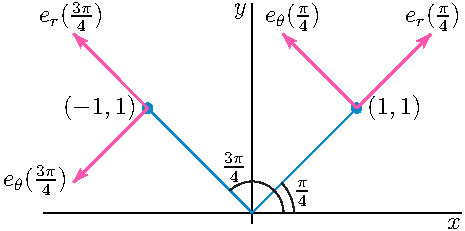
\includegraphics{polar2.pdf}
\end{center}
\end{solution}

%%%%%%%%%%%%%%%%%%%%%%%%%%%%%%%%
\begin{question}[M200 2008A] %7
Match the following equations with the corresponding 
pictures. Cartesian coordinates are $(x, y)$ and polar coordinates are 
$(r, \theta)$.

\begin{center}
 (A) \raisebox{-0.5\height}
           {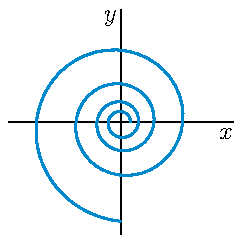
\includegraphics[width=0.33\textwidth, height=0.3\textwidth]
                                                   {polarCurveE.pdf}}
\qquad
  (B) \raisebox{-0.5\height}
            {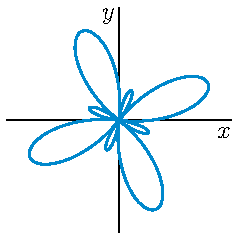
\includegraphics[width=0.33\textwidth, height=0.33\textwidth]
                                                   {polarCurveB.pdf}}
\end{center}
\begin{center}
  (C) \raisebox{-0.5\height}
            {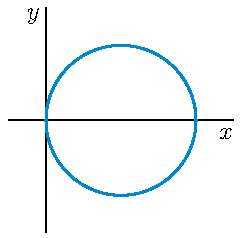
\includegraphics[width=0.33\textwidth, height=0.33\textwidth]
                                                   {polarCurveC.pdf}}
\qquad
  (D)  \raisebox{-0.5\height} 
            { 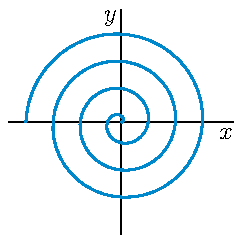
\includegraphics[width=0.33\textwidth, height=0.3\textwidth]
                                                    {polarCurveF.pdf}}
\end{center}
\begin{center}
 (E) \raisebox{-0.5\height}
           { 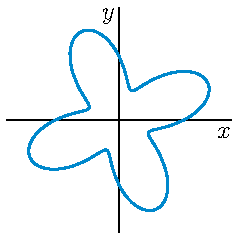
\includegraphics[width=0.33\textwidth, height=0.3\textwidth]
                                                    {polarCurveA.pdf}}
\qquad
  (F) \raisebox{-0.5\height}
           {  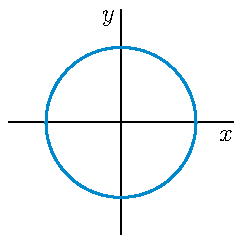
\includegraphics[width=0.33\textwidth, height=0.3\textwidth]
                                                    {polarCurveD.pdf}}
\end{center}

\begin{alignat*}{7}
&\text{(a)}\quad& r&=2+\sin(4\theta) \qquad\qquad &
&\text{(b)}\quad& r&=1+2\sin(4\theta)\qquad\qquad &
&\text{(c)}\quad& r&=1\\
&\text{(d)}& r&=2\cos(\theta),\ 
           -\tfrac{\pi}{2}\le\theta\le\tfrac{\pi}{2}\qquad\qquad &
&\text{(e)}& r&=e^{\theta/10}+e^{-\theta/10}\qquad\qquad &
&\text{(f)}& r&=\theta &
\end{alignat*}
\end{question}

%\begin{hint}
%
%\end{hint}

\begin{answer}
(a) $\leftrightarrow$ (E) \qquad
(b) $\leftrightarrow$ (B) \qquad
(c) $\leftrightarrow$ (F) \qquad
(d) $\leftrightarrow$ (C) \qquad
(e) $\leftrightarrow$ (A) \qquad
(f) $\leftrightarrow$ (D)
\end{answer}

\begin{solution}
(a) Since $-1\le \sin(4\theta)\le 1$, the coordinate $r=2+\sin(4\theta)$ oscillates between $r=1$ and $r=3$ as $\theta$ runs from $0$ to $2\pi$.
The maximum value $r=3$ is achieved when $\sin(4\theta)=1$, i.e when
$4\theta=\frac{\pi}{2} +2n\pi$, i.e. when $\theta=\frac{\pi}{8}+\frac{n\pi}{2}$.
That matches figure (E).

(b) Since $-1\le \sin(4\theta)\le 1$, the coordinate $r=1+2\sin(4\theta)$ takes its maximum value $r=3$ when $\sin(4\theta)=1$, i.e. when $\theta=\frac{\pi}{8}+\frac{n\pi}{2}$, just as the case with $(a)$. But now
$r$ can also take the value $0$. That matches figure (B).

(c) $r=1$ is completely indepedent of $\theta$. All points on the curve $r=1$
are a distance $1$ from the origin. That is, $r=1$ is the circle of radius $1$
centred on the origin. That's figure (F).

(d) In this case, $\theta$ is subject to the restriction 
$-\frac{\pi}{2}\le\theta\le\frac{\pi}{2}$, like figure (C).
Figure (C) looks like a circle. We can verify that $r=2\cos(\theta)$ is 
indeed a circle by converting to Cartesian coordinates. We can convert the right hand side to exactly $2x=2r\cos(\theta)$ by multiplying the 
whole equation by $r$.
\begin{align*}
r=2\cos(\theta)
&\iff r^2 =2r\cos(\theta)
\iff x^2+y^2=2x \\
&\iff (x-1)^2+y^2=1
\end{align*}
So $r=2\cos(\theta)$ is the circle of radius $1$ centred on $x=1$, $y=0$,
which indeed matches figure (C).

(e) When $\theta=0$, $r=e^{\theta/10}+e^{-\theta/10}=2$.
As 
\begin{equation*}
\diff{}{\theta}\big(e^{\theta/10}+e^{-\theta/10}\big)
    =\frac{1}{10}\big(e^{\theta/10}-e^{-\theta/10}\big)
    >0\qquad\text{for all }\theta > 0
\end{equation*}
$r=e^{\theta/10}+e^{-\theta/10}$ increases as $\theta$ increases for all
$\theta\ge 0$. Furthermore the rate of increase gets bigger and bigger as 
$\theta$ gets bigger and bigger. So $r$ starts at $r=2$ when $\theta=0$
and increases faster and faster as $\theta$ increases. That matches figure (A).

(f) When $\theta=0$, $r=\theta=0$.
As 
\begin{equation*}
\diff{}{\theta} \theta
    =1 \qquad\text{for all }\theta
\end{equation*}
$r=\theta$ increases as $\theta$ increases for all
$\theta\ge 0$. Furthermore the rate of increase is independent of $\theta$.
So $r$ starts at $r=0$ when $\theta=0$
and increases at a constant rate as $\theta$ increases.
That matches figure (D).

\end{solution}


%%%%%%%%%%%%%%%%%%
\subsection*{\Procedural}
%%%%%%%%%%%%%%%%%%

%%%%%%%%%%%%%%%%%%%%%%%%%%%
\begin{question}\label{prb polar curvature}
Recall that a point with polar coordinates $r$ and
$\theta$ has $x=r\cos\theta$ and $y=r\sin\theta$. Let $r=f(\theta)$ be 
the equation of a plane curve in polar coordinates. Find the 
curvature of this curve at a general point $\theta$. 
\end{question}

\begin{hint} 
The curve can be parametrized by 
$\vr(\theta)= f(\theta)\big[\cos\theta\ \hi + \sin\theta\ \hj\big]$
\end{hint}

\begin{answer} 
$\ka(\theta)=\frac{\big|f(\theta)^2+2f'(\theta)^2-f(\theta)f''(\theta)\big|}
                     {{[f(\theta)^2+f'(\theta)^2]}^{3/2}}$
\end{answer}


\begin{solution}
Think of $\theta$ as a time parameter and recall that
$\ka(\theta)=\frac{|\vv(\theta)\times\va(\theta)|}{|\vv(\theta)|^3}$.
The given curve has
\begin{align*}
x(\theta)&= f(\theta)\cos\theta\\
y(\theta)&= f(\theta)\sin\theta \\
\vr(\theta)&= f(\theta)\big[\cos\theta\ \hi + \sin\theta\ \hj\big] \\
\vv(\theta)=\vr'(\theta)&= f'(\theta)\big[\cos\theta\ \hi + \sin\theta\ \hj\big]
          +f(\theta)\big[-\sin\theta\ \hi + \cos\theta\ \hj\big] \\
\va(\theta)=\vr''(\theta)&= \big\{f''(\theta)-f(\theta)\big\}\big[\cos\theta\ \hi + \sin\theta\ \hj\big]
             +2f'(\theta)\big[-\sin\theta\ \hi + \cos\theta\ \hj\big]  
\end{align*}
The efficient way to compute $|\vv(\theta)|$ and
the cross product $\vv(\theta)\times\va(\theta)$
is to observe that
\begin{align*}
\vv(\theta)&= f'(\theta)\,\he_r(\theta) +f(\theta)\,\he_\theta(\theta) \\
\va(\theta)&= \big\{f''(\theta)-f(\theta)\big\}\,\he_r(\theta)
             +2f'(\theta)\,\he_\theta(\theta)
\end{align*}
where $\he_r(\theta)$ and $\he_\theta(\theta)$ are the vectors of
Q[\ref{prb polar vectors}].  As $\he_r(\theta)$ and $\he_\theta(\theta)$
are mutually perpendicular unit vectors
obeying $\he_r(\theta)\times\he_\theta(\theta) =\hk$ and 
$\he_r(\theta)\times\he_r(\theta) = \he_\theta(\theta)\times\he_\theta(\theta) =0$,
\begin{align*}
|\vv(\theta)|^2=\vv(\theta)\cdot\vv(\theta)
   &=\big[f'(\theta)\,\he_r(\theta) +f(\theta)\,\he_\theta(\theta)\big]\cdot
     \big[f'(\theta)\,\he_r(\theta) +f(\theta)\,\he_\theta(\theta)\big] \\
   &=f'(\theta)^2\,\he_r(\theta)\cdot\he_r(\theta)
     +f(\theta)^2\,\he_\theta(\theta)\cdot\he_\theta(\theta)
     +2f'(\theta)\,f(\theta)\,\he_r(\theta)\cdot\he_\theta(\theta) \\
   &=f'(\theta)^2+f(\theta)^2  \\
|\vv(\theta)|& = \sqrt{f'(\theta)^2+f(\theta)^2}\\
\vv(\theta)\times\va(\theta) 
 &=\big[f'(\theta)\,\he_r(\theta) +f(\theta)\,\he_\theta(\theta)\big]\times
   \big[\big\{f''(\theta)-f(\theta)\big\}\,\he_r(\theta)
             +2f'(\theta)\,\he_\theta(\theta)\big] \\
 &= 2f'(\theta)^2\,\he_r(\theta)\times\he_\theta(\theta)
  +f(\theta)[f''(\theta)-f(\theta)]\,\he_\theta(\theta)\times\he_r(\theta)
                                \\
 &= \big\{2f'(\theta)^2-f(\theta)[f''(\theta)-f(\theta)]\big\}
                                \,\hk
\end{align*}
So
\begin{align*}
\ka(\theta)&=\frac{|\vv(\theta)\times\va(\theta)|}{|\vv(\theta)|^3}
=\frac{\big|f(\theta)^2+2f'(\theta)^2-f(\theta)f''(\theta)\big|}
                     {{[f(\theta)^2+f'(\theta)^2]}^{3/2}}
\end{align*}
\end{solution}



%%%%%%%%%%%%%%%%%%%%%%%%%%%
\begin{question}
Find the curvature of the cardioid $r=a(1-\cos\theta)$.
\end{question}

%\begin{hint} 
%\end{hint}

\begin{answer} 
$\ka(\theta)=\frac{3}{2^{3/2}a\sqrt{1-\cos\theta}}
   =\frac{3}{2\sqrt{2ar(\theta)}}$
\end{answer}


\begin{solution}
By the Q[\ref{prb polar curvature}] with
\begin{align*}
f(\theta)  = a(1-\cos\theta)\qquad
f'(\theta) = a\sin\theta\qquad
f''(\theta) =a\cos\theta
\end{align*}
we have
\begin{align*}
\ka(\theta)
&=\frac{\big|f(\theta)^2+2f'(\theta)^2-f(\theta)f''(\theta)\big|}
                     {[f(\theta)^2+f'(\theta)^2]^{3/2}}\\
&=\frac{\big|a^2-2a^2\cos\theta+a^2\cos^2\theta+2a^2\sin^2\theta-
                a^2\cos\theta+a^2\cos^2\theta\big|}
        {[a^2-2a^2\cos\theta+a^2\cos^2\theta+a^2\sin^2\theta]^{3/2}}\\
&=\frac{3a^2-3a^2\cos\theta}{[2a^2-2a^2\cos\theta]^{3/2}}
=\frac{3}{2^{3/2}a\sqrt{1-\cos\theta}}
=\frac{3}{2\sqrt{2ar(\theta)}}
\end{align*}
\end{solution}

%%%%%%%%%%%%%%%%%%
%\subsection*{\Application}
%%%%%%%%%%%%%%%%%%








